%!TEX root = ../csuthesis_main.tex

\section{绪论} \label{section:one}

\subsection{研究背景与意义}
音频信号承载着丰富的语义信息与环境状态——从一段录音中，我们不仅能分辨出"谁在说话"，还能推断出说话的场景、情绪乃至周边发生的事件。让机器自动完成这种从波形到语义类别的映射，正是音频分类的核心任务。近十年来，物联网终端、可穿戴传感器和边缘计算节点的爆发式部署，催生了对轻量化音频理解能力的刚性需求\citess{gourisaria2024comparative}。这项技术已渗透到多个关键行业：医疗领域，智能听诊器不间断地监听心肺音，医生借此捕捉早期病变信号\citess{medical2026synthetic, heart2025mfcc}；工业线上，齿轮箱或轴承的细微异响一旦被算法捕获，就能在停机前触发预警，省去高昂的抢修成本\citess{hafiz2025machine, wang2021unsupervised}；安防场景中，系统需要从嘈杂的背景声中分离出玻璃碎裂或呼救声，这要求模型具备极强的抗噪判别力\citess{crocco2016audio, foggia2015audio}；海洋工程里，被动声呐在混响和水流噪声的干扰下识别水下目标，深度学习正逐步替代传统的人工听判流程\citess{xu2024underwater}。可以说，音频分类已不再是一个孤立的算法问题，而是构成了现代感知系统中不可或缺的底层能力。

然而，边缘环境在部署时通常面临严格的物理限制。功耗约束、计算资源短缺以及响应延迟要求，均对底层算法的轻量化提出了挑战。回顾技术演进，早期的音频处理主要依赖数字信号处理技术。例如提取梅尔频率倒谱系数（MFCC），再结合支持向量机等传统机器学习模型进行模式识别\citess{tzanetakis2002musical}。此类方法存在较强的专家先验依赖，在面对非平稳信号或复杂噪声时，浅层统计模型的表征能力与泛化性能往往受限。为突破手工特征设计的局限，深度学习逐渐成为该领域的主流，实现了端到端的特征提取\citess{purwins2019deep}。目前常见的方案是利用卷积神经网络（CNN）提取局部时频纹理，配合循环神经网络（RNN）进行时序规律建模\citess{hershey2017cnn, kong2020panns, cakir2017crnn, Rezaul2024}。虽然增加网络层数有效提升了分类精度，但这同时导致了模型参数量与算力开销的显著增加。面对高维时序数据，庞大的网络结构难以适应边缘节点的计算环境，经典冯·诺依曼架构的算力局限也日益凸显\citess{chen2023complexity, arute2019quantum}。

面对经典计算在算力与功耗方面的局限，量子计算理论提供了一种具有潜力的解决途径。其理论基础在于利用量子比特的叠加与纠缠机制，在希尔伯特空间完成高维特征映射\citess{bharti2022noisy, havlivcek2019supervised}。相关研究证实，依托 NISQ 设备，轻量级的参数化量子线路能够在较低参数量下维持一定的特征提取能力\citess{shi2025nisq, huang2018survey}。这种高参数效率的物理特性，与边缘音频分类任务对模型轻量化的需求较为契合。近年来，已有研究尝试将量子机器学习应用于声学数据分析\citess{henderson2020quanvolutional}。然而，现有的量子音频分类模型在实际应用中仍面临以下两方面问题：
（1）时序特征难以有效保留：主流的量子数据编码方法通常侧重于静态特征的映射，难以充分表征音频信号的时间演化特性\citess{larose2020robust, schuld2019quantum}，容易在量子态制备阶段造成核心时序信息的流失。
（2）模型训练收敛困难：受当前 NISQ 设备硬件噪声的影响，深层参数化量子线路在优化过程中易出现“贫瘠高原”现象。该现象本质上是指损失函数在参数空间的梯度方差随系统规模呈指数级衰减，表现为搜索景观极其平坦，导致经典优化器因无法获取有效的更新方向而陷入优化停滞，增加了模型的训练与收敛难度。

针对上述经典音频分类模型因参数规模庞大导致的高算力开销，以及现有量子模型在时序特征保留与网络训练收敛方面存在的双重局限，本文研究聚焦于音频分类任务需求，开展了面向音频时序特征的量子时频分析神经网络及其优化机制研究。具体来说，本文针对传统量子编码方式侧重于静态特征映射、难以有效捕获音频信号随时间变化的动态演化特征的局限，提出了一种基于双量子比特序列纠缠的量子时序编码方法，旨在确保音频特征在映射至量子空间后仍能保持完备的时频关联结构；同时，针对含噪中等规模量子设备下参数化线路的优化停滞痛点，提出了跨计算范式的训练方法，旨在保障极低参数限制下音频分类算法的寻优效率与识别有效性。综上所述，本文工作不仅在理论上为量子机器学习处理复杂非平稳信号提供了探索路径，更在实际应用中为物联网等低功耗环境下的音频分类与识别任务提供了关键的轻量化算法支撑。

\subsection{国内外研究现状}
音频分类技术的发展经历了一个渐进的演化过程。近期的研究跨度涵盖了人工特征工程、经典深度神经网络，以及前沿的量子计算范式。探讨视角主要分为四个维度：音频分类任务的技术演进、量子信息的编码规则、量子神经网络架构的设计，以及模型压缩领域的知识蒸馏技术。

\subsubsection{音频分类任务}

音频分类的核心在于解析连续的音频波形，提取关键的时频与声学特征，并将其映射至相应的语义类别。其发展历程主要分为三个阶段：浅层统计模型时期、深层神经网络时期，以及当前处于探索阶段的轻量化量子模型时期。

在浅层统计模型时期，受限于当时的计算资源与理论框架，音频分类的特征提取高度依赖专家先验知识。研究者们构建了诸如短时傅里叶频谱（STFT）、线性预测编码（LPC）以及梅尔频率倒谱系数（MFCC）等经典声学特征\citess{chowdhury2019fusing}，旨在利用严密的数学与物理模型高保真地近似人耳的非线性听觉感知。这类基于心理声学的特征工程，在早期的孤立词语音识别、基础乐器检测以及纯净环境下的音乐流派分类等任务中确立了早期的行业标准。获取这些离散特征后，系统通常会将其送入支持向量机（SVM）、隐马尔可夫模型（HMM）或高斯混合模型（GMM）等传统统计算法中进行模式匹配\citess{tzanetakis2002musical}。客观而言，此类级联范式在受控且平稳的声学环境中取得了奠基性的成效。然而，面对真实场景中高度非平稳的复杂音频流（如多声源混叠、剧烈波动的环境底噪等）时，其局限性日益凸显。一方面，这种将特征提取与分类决策相割裂的“两阶段”处理机制，阻断了梯度反馈，使得系统无法进行端到端的全局联合优化\citess{ouisaadane2024experiment}；另一方面，由于后端的浅层统计模型缺乏高维非线性映射能力，难以充分捕捉连续声学帧之间的动态演化规律\citess{ding2024acoustic}。这种表征上限与拓扑结构的双重受限，导致其在复杂序列感知任务中的泛化性能始终难以取得实质性突破，存在明显的理论瓶颈。

进入2010年代中后期，随着GPU并行计算能力的提升与大规模音频数据集的开源，音频处理逐渐向端到端的深层神经网络时期转变。图\ref{AC_Process}展示了一个典型的现代音频识别分类流程：一维音频波形通常被预处理为二维声谱图或梅尔对数频谱图，随后输入神经网络进行高维特征提取。2017年，Hershey等人\citess{hershey2017cnn}验证了将二维卷积神经网络直接应用于音频时频图以提取局部纹理与能量分布特征的有效性。为进一步提取时间轴上的长距离上下文依赖，Cakir等人\citess{cakir2017crnn}同年提出了卷积循环神经网络，该架构前端利用CNN提取局部频谱特征，后端结合循环层对帧级别的动态演化规律进行时序建模。2020年，Kong等人\citess{kong2020panns}提出的PANNs（预训练音频神经网络）架构，系统评估了从VGG到ResNet等不同深度网络在多类音频模式识别中的表现，进一步证实了增加网络深度能够显著扩大感受野，从而提升复杂声学事件的识别率。

\begin{figure*}[htpb]
	\centering
	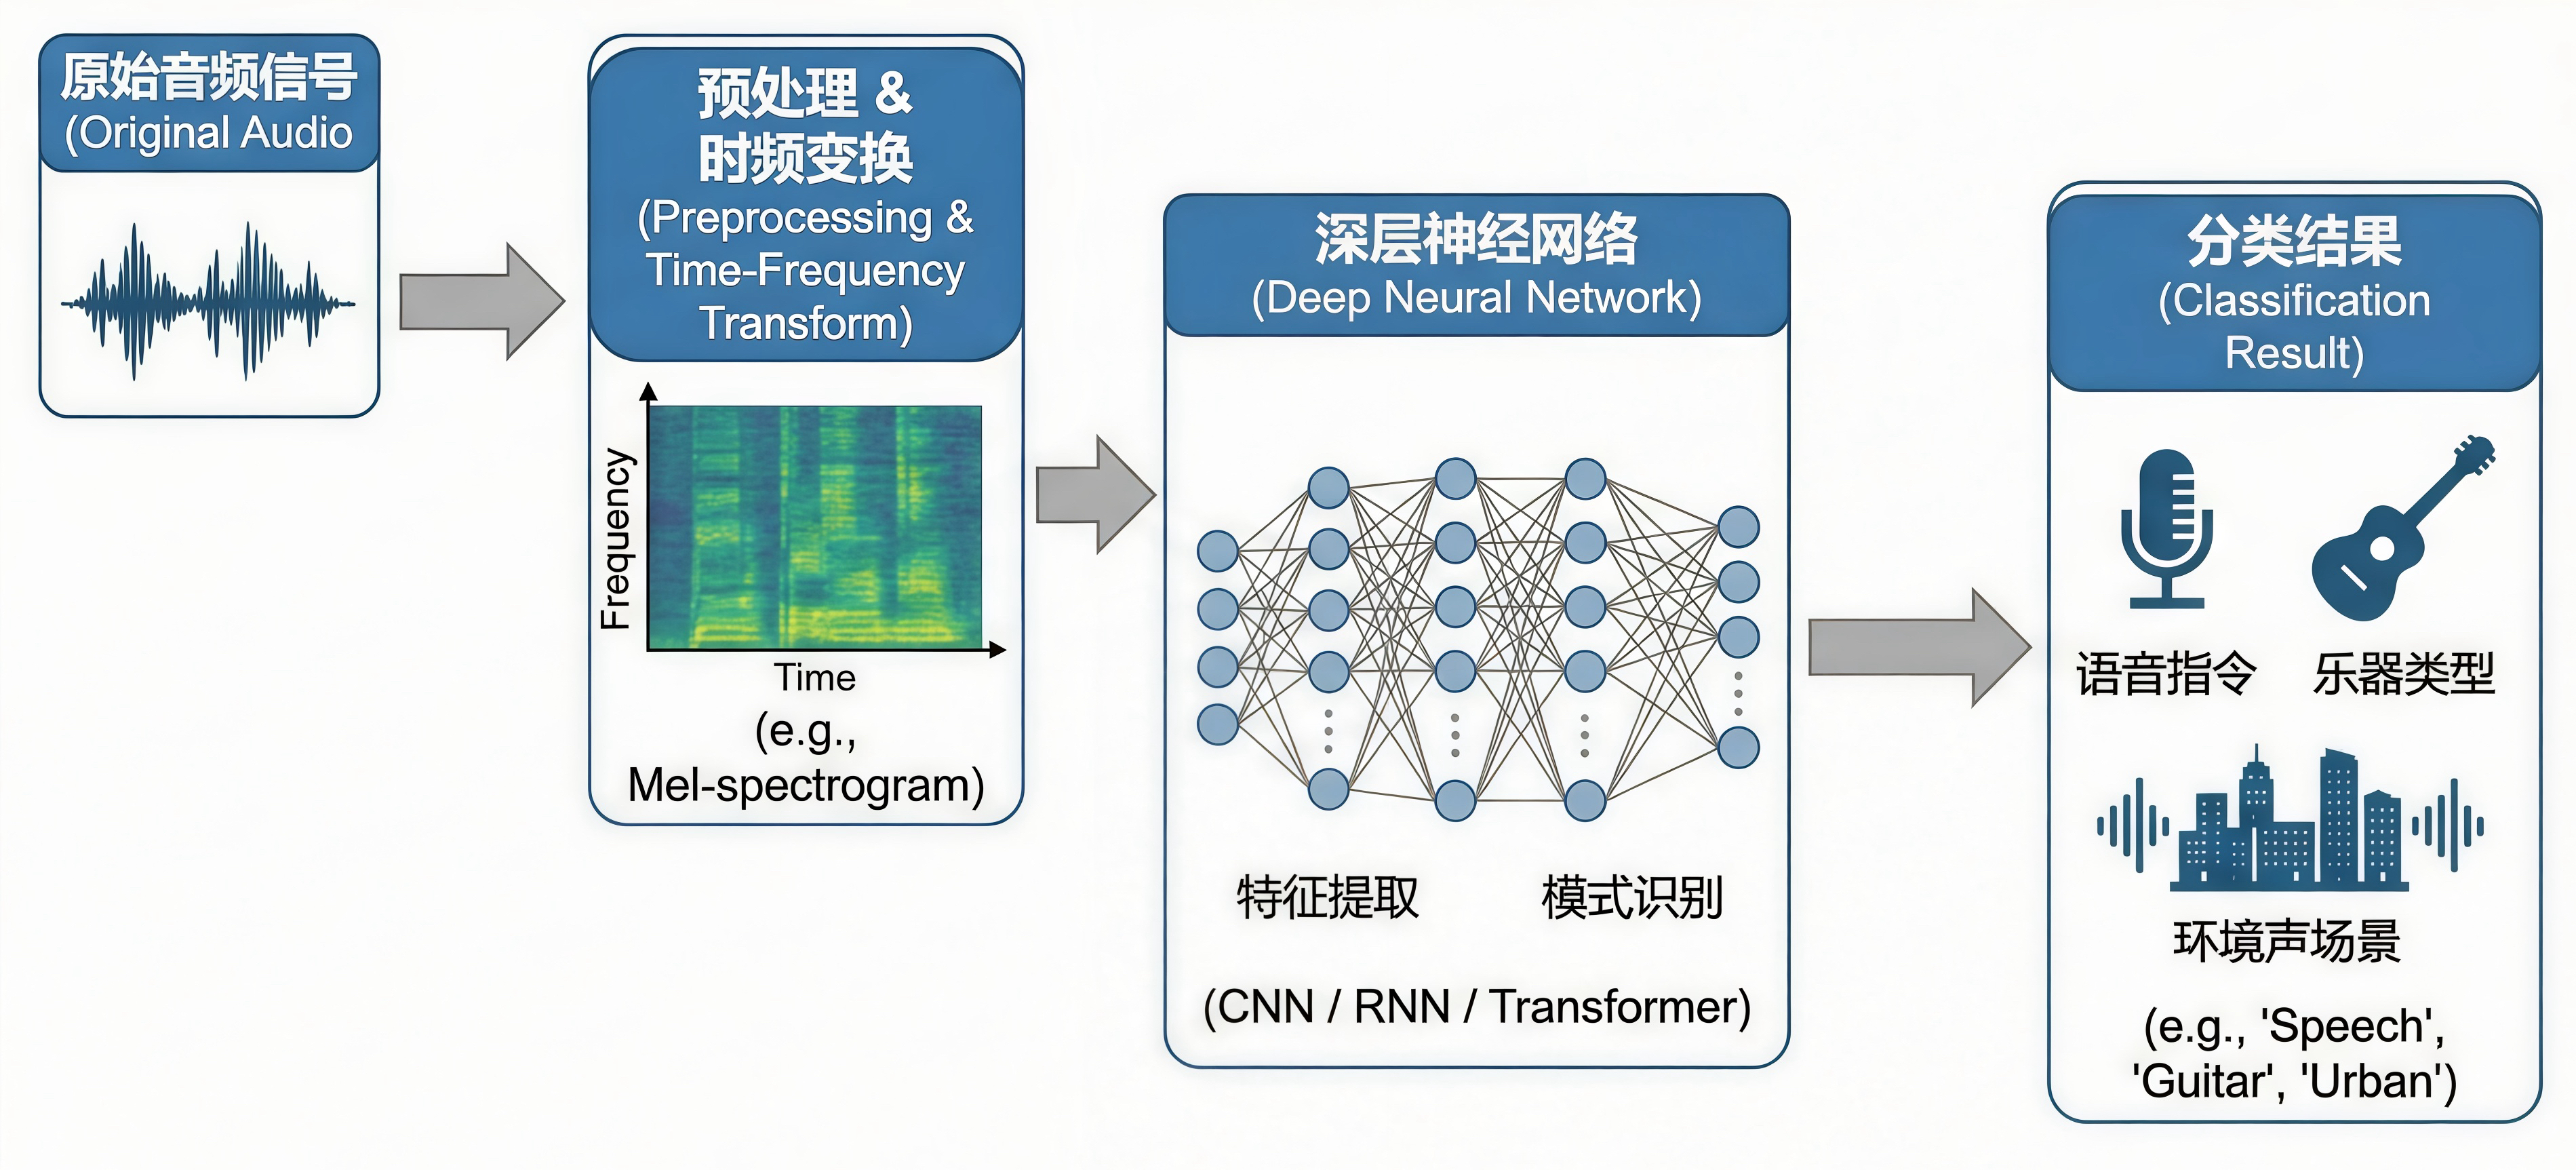
\includegraphics[width=0.8\textwidth, keepaspectratio]{./images/chapter1/AC_Process.jpg}
	\caption{音频识别分类流程示例图}
	\label{AC_Process}
\end{figure*}


为克服浅层线路的表征局限，学术界率先转向架构优化与特征适配。例如，2023年 Lourens 等人\citess{lourens2023hierarchical}将神经架构搜索（NAS）引入量子音频领域以自动化构建变分线路；Rezaul 等人\citess{Rezaul2024}则探讨了混合计算范式下的特征维度缩减策略。然而，这些早期探索多侧重于静态空间维度的频谱压缩，未能充分捕捉声学事件在时间轴上的演化规律，导致显式动态时序建模的缺失成为限制性能提升的核心瓶颈。近年来，这一局限正被一系列前沿研究所突破。2025年，Agarwal 等人开发的 QuantumMelody 系统通过在量子线路中联合编码多维声学特征，初步验证了混合范式在复杂音频时序任务中的潜力\citess{agarwal2025quantum}；Yan 等人则针对 NISQ 设备的硬件约束，利用创新损失函数设计了高稳定性的框架，有效增强了模型对语音时间结构的恢复能力\citess{yan2025quantum}。为进一步突破人工设计线路的性能上限，Kashif 等人在2025年提出了 FAQNAS 框架，在硬件约束下实现了量子网络处理音频时序特征的自动化寻优\citess{kashif2025faqnas}。随着研究的深化，2026年 Qi 等人引入张量列（Tensor-Train）编码技术对高维信号进行低秩表示，有效缓解了长时音频流处理中的灾难性遗忘问题\citess{qi2026continual}。上述代表性工作标志着量子音频处理正从静态空间映射向显式动态时序建模发生关键的范式转变。尽管如此，这些前沿方案往往高度依赖极其昂贵的架构搜索算力或复杂的混合演化策略；如何在保持极低、固定参数规模的前提下，设计出能高保真保留音频动态规律的量子时序编码机制，并突破深层线路的寻优瓶颈，仍是当前该领域亟待攻克的核心痛点。

\subsubsection{量子信息的编码与表示}

在量子机器学习的完整工作流中，量子信息编码是将经典实数向量转换为量子希尔伯特空间中可计算量子态的过程。该环节直接决定了后续量子特征提取电路的表达上限。编码技术经历了从追求极致空间压缩比的基础方法，向适应 NISQ 设备硬件友好型机制，再到近期初探动态时序映射的演进。

在早期研究中，常采用基态编码和振幅编码。2014年，Schuld等人\citess{schuld2014quantum}论述了振幅编码方法，该方法通过将归一化后的$N$维数据精确映射到$\log_2 N$个量子比特的概率幅上，理论上能够实现指数级别的数据压缩比。然而，振幅编码所需的量子态制备线路深度与数据维度呈线性正相关，在现有物理设备上极易受到环境噪声影响而产生退相干效应，导致信息失真。针对多媒体数据的结构化特征，Wang等人\citess{wang2016qrda}于2016年提出了量子数字音频表示法（QRDA），利用两组相互纠缠的量子比特序列分别对音频信号的采样时间戳坐标和信号幅度信息进行编码。2018年，Yan等人\citess{YAN201871}在QRDA的基础上提出了多通道量子音频表示（MCQA），通过引入额外的控制通道量子比特，实现了多路立体声信号的同步纠缠存储与基本仿射变换。

为降低制备线路的门复杂度与噪声敏感度，角度编码得到了广泛应用。LaRose等人\citess{larose2020robust}在2020年的研究中系统评估了角度编码在变分量子分类器中的表现。该方法将经典特征向量直接作为旋转量子门（如$R_x, R_y, R_z$）的相位角度参数。虽然角度编码所需量子比特数通常与输入特征维度相同（$O(N)$），不具备空间压缩优势，但因其制备线路深度为常数级（$O(1)$），表现出较好的抗噪鲁棒性，成为该时期变分量子算法中较为普遍的编码选择。

随着量子机器学习应用场景从静态图像向非平稳时间序列扩展，传统静态编码方式的局限性被充分暴露。正如近期关于NISQ设备混合架构的系统性综述\citess{shi2025nisq}所指出的，量子模型在处理复杂感知任务时的性能瓶颈，很大程度上源于前端编码机制无法有效映射数据的时空拓扑结构。为突破这一局限，2025年以来的前沿研究开始探索动态量子编码策略。例如，Agarwal 等人\citess{agarwal2025quantum}尝试在模拟量子线路中通过分组机制对多维声学特征（音高、力度等）进行联合相位编码，初步实现了异构特征的量子态集成；Qi 等人\citess{qi2026continual}则深入量子态的代数结构，开发了张量列（Tensor-Train）编码技术，通过将高维随机时序信号压缩为低秩量子特征表示，在编码阶段有效保留了序列数据的长程时序依赖。这些前沿探索代表了量子信息编码从“单纯空间压缩”向“时序拓扑保留”的重要理论跨越。然而，聚焦于边缘计算与NISQ设备的严苛资源约束，现有方案在落地时仍面临客观的物理瓶颈。无论是依赖高门复杂度的早期结构化表示，还是依赖密集经典预处理的高阶张量网络，均难以在极低功耗下实现高效的梯度反馈与时频信息纠缠。因此，如何跳出繁杂的经典数据降维逻辑，设计一种兼具极浅制备线路与原生时序纠缠能力的轻量级编码范式，构成了当前算法构建中亟待突破的核心难点。

\subsubsection{量子神经网络}  

量子神经网络（QNN）结合了经典神经网络的非线性函数拟合能力与量子计算的高维希尔伯特空间并行优势。其发展经历了早期物理模型构建、基于 NISQ 设备的变分架构应用以及可训练性分析的优化阶段。

在早期阶段，研究主要集中于理论基础与物理机制推演。1996年，Behrman等人\citess{behrman1996quantum}构建了模拟经典逻辑门操作的量子点分子动态数学模型；Tóth等人\citess{toth1996quantum}提出了基于近邻自旋耦合相互作用的量子细胞自动机结构；Lewenstein\citess{Lewenstein01121994}于1994年定义了“量子感知机”概念，将其表述为通过一系列幺正变换演化输入量子态并进行可观测测量的计算单元，为QNN的算法设计提供了理论参考。

随着 NISQ 设备的发展，变分量子算法框架得到了广泛应用。2016年，McClean等人\citess{mcclean2016theory}与2021年Cerezo等人\citess{cerezo2021variational}的研究推动了该混合优化框架的建立。2019年，Benedetti等人\citess{benedetti2019parameterized}表明，通过构建参数化量子线路，可利用经典优化算法迭代更新量子门参数，进而实现最优特征映射。国内学者Huang等人\citess{huang2018survey}指出，量子机器学习算法在处理大规模参数空间时具有潜在的并行搜索优势。在此基础上，Cong等人\citess{cong2019quantum}于2019年提出了量子卷积神经网络（QCNN）。该架构利用局部的两比特或三比特参数化量子门模拟经典感受野，并通过测量部分量子比特来模拟空间池化机制，有效降低了系统的总维度。同期，陈佳临等人\citess{chen2019qnn}提出的量子并行神经网络，探讨了利用量子态叠加性质提升网络隐层节点特征存储容量的可行性。

在尝试增加QNN网络深度与量子比特数以处理高维复杂任务时，“贫瘠高原”现象成为主要的优化瓶颈\citess{mcclean2018barren}。该现象表明，在随机初始化的深层参数化线路中，损失函数相对于任意参数的梯度方差随量子比特数量增加而呈指数级衰减，导致经典优化器无法获取有效的更新方向。针对梯度消失问题，2024年Liao等人\citess{liao2024quantum}尝试将损失函数的全局信息通过相干编码技术映射至参数空间的量子叠加态中，以探索从物理层面试图平滑优化景观的方法。

结合经典算力的混合框架成为应对硬件限制的主要研究路径\citess{shi2025nisq}。研究更加侧重于模型鲁棒性验证与特定物理任务下的微架构设计。2025年，Shi等人\citess{shi2025quantest}提出了“QuanTest”框架，利用量子纠缠充分性准则自动生成测试样本，以量化评估QNN线路内部的表达缺陷；Tabarraei\citess{sukulthanasorn2026quantum}在2025年的工作中，将变分量子线路与坐标神经解码架构相结合用于结构拓扑优化，实验表明量子编码在特定边界条件下相比经典方案具有更高的参数效率与设计多样性，证实了浅层参数化量子线路在不涉及时间变量的静态优化任务中的应用潜力。然而，现有包含QCNN在内的主流架构多作为静态空间特征提取器运作，系统状态随时间演化的哈密顿动力学机制未能有效融合于分类任务中，因此在处理音频等具备长程时间依赖性的感知任务时，仍表现出表征能力的不足。

\subsubsection{模型压缩与知识蒸馏}

为解决深度预训练模型参数量级过大以及在端侧设备部署受限的问题，模型轻量化技术得到了系统性发展，并随着混合计算框架的普及，逐渐从经典计算领域延伸至量子机器学习领域。

在轻量化技术发展早期，知识蒸馏主要应用于纯经典计算环境。自深度学习学者Hinton等人\citess{hinton2015distilling}于2015年系统化地提出该方法以来，其核心机制在于：引入一个带有温度超参数的Softmax函数，利用参数量庞大、泛化能力强的“教师”网络输出的软标签（包含类别间相似性的暗知识），计算与紧凑型“学生”网络输出分布之间的相对熵（KL散度），从而指导学生网络进行优化。这一机制已成为模型轻量化的标准技术路径。

相关研究开始探讨将此种轻量化方法引入量子网络。2022年，Shao等人\citess{shao2022knowledge}在相关综述中分析了知识蒸馏技术在量子神经网络中的适用性，指出该方法通过联合损失函数的设定，有望实现跨模态或跨网络层级的特征迁移，并有助于在维持分类性能的同时降低量子模型对线路深度和物理逻辑比特数的需求。

直接面向量子线路的压缩与微调技术取得了一定数学理论层面的进展。在线路剪枝方面，LiePrune 方法\citess{lieprune2025}利用量子线路底层的李群代数同构性质，对构成冗余演化的参数化量子门进行有效剪除；此外，基于量子参数生成的微调方法\citess{qpa2025quantum}，表明可以在冻结大部分线路结构、维持模型基础表征性能的前提下，实现可训练参数规模的多项式甚至对数级缩减，从而提升QNN在相干时间受限的NISQ设备上的运行可行性。

纯量子体系内的蒸馏与跨计算范式蒸馏成为前沿研究课题。Yan等人\citess{yan2026distilling}在2026年提出了一种面向量子神经网络的原生知识蒸馏框架，论证了利用保真度或迹距离度量，将深层量子教师线路的状态演化知识转移至浅层量子学生模型的可行性。在跨范式知识迁移方面，为了充分利用经典架构的成熟算力红利，Hasan等人\citess{hasan2023bridging}提出了“经典-量子混合蒸馏”方案。该方案使用在海量数据上预训练的经典大参数CNN作为教师模型，通过温度缩放的软标签蒸馏损失（KL散度），指导参数量较少（通常在数十个参数级别）的量子变分网络学习教师输出概率分布中包含的暗知识。这种跨范式方法利用经典网络收敛后的优化结果辅助量子模型的参数更新，为缓解量子参数空间中的“贫瘠高原”现象提供了不同维度的研究思路。然而，当前跨范式蒸馏策略的损失函数设计多集中于静态图像的空间语义特征对齐。针对具有非平稳时间序列特性的音频分类任务，如何构建能够有效传递经典CNN/RNN结构中“长程时序动态依赖”和“时频演化规律”的经典-量子联合蒸馏机制，仍是当前研究中有待填补的空白。

\subsection{论文的主要工作与创新点}

本论文通过结合量子计算理论、音频信号处理以及深度学习技术，探索量子计算在音频分类领域的应用潜力。主要的研究内容在于构建量子时频分析神经网络，详细介绍其基本原理以及在音频分类任务中的运用。针对现有量子音频处理方法中存在的时序特征丢失、参数利用率低以及在NISQ设备上训练困难等问题，本文提出了一种基于时序编码的量子神经网络音频分类方案及其优化对策。

本文的研究动机、主要工作内容与总体目标如图\ref{Motivation_Flowchart}所示。面对经典深度学习在参数与算力上的瓶颈，以及现有量子方法忽略时序特性且在NISQ设备上深层线路训练困难的挑战，本文确立了“面向动态时序特征的量子时频分析神经网络与优化研究”这一核心命题。围绕该命题，本文重点开展了三项递进式研究：基于量子时序编码的音频特征表示、量子时频分析神经网络模型构建，以及跨计算范式的经典-量子知识蒸馏。最终旨在构建高参数效率的量子架构，克服贫瘠高原现象，全面提升音频分类的准确率与鲁棒性。

\begin{figure*}[htpb]
	\centering
	% 请确保图片路径和文件名与你实际保存的一致
	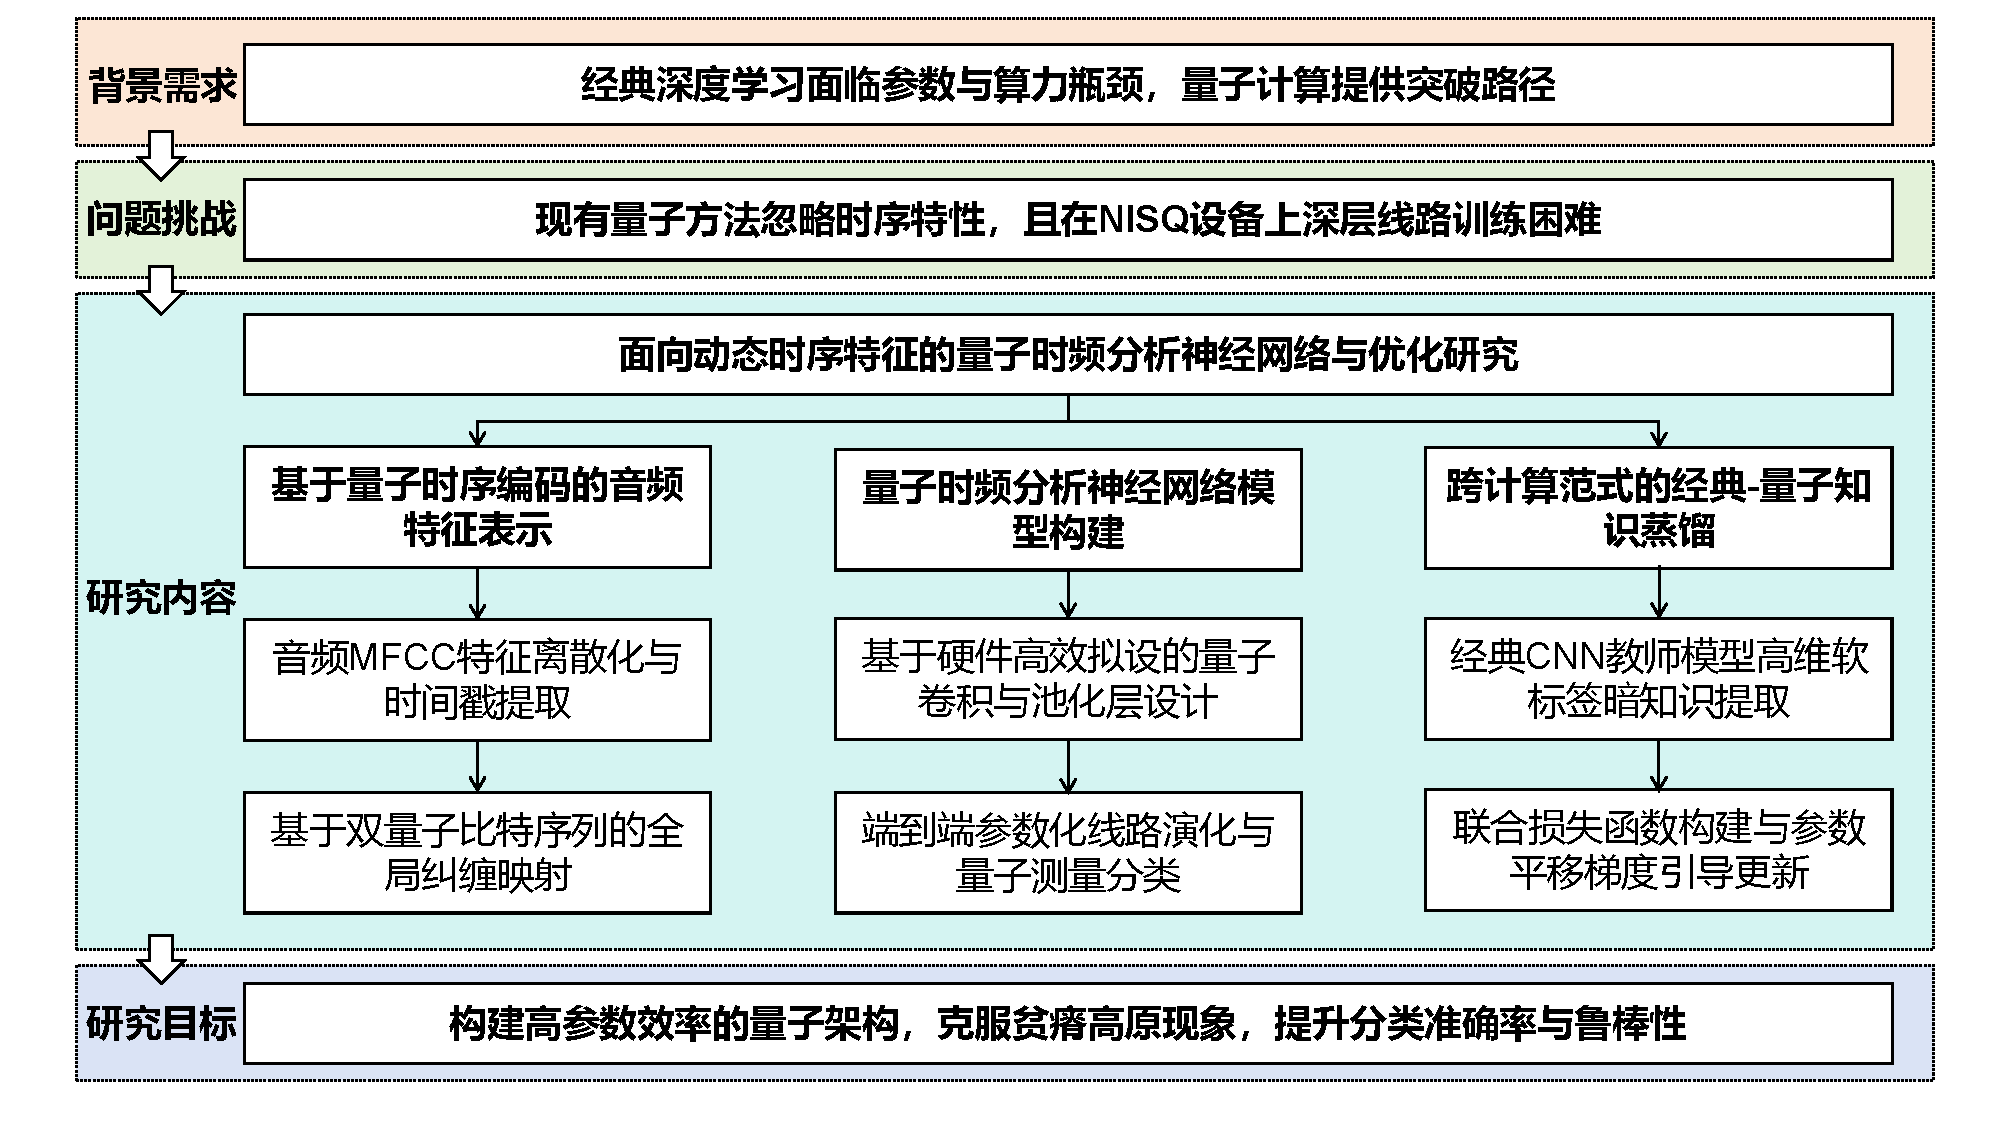
\includegraphics[width=1\textwidth, keepaspectratio]{./images/Research_Motivation.pdf}
	\caption{本文研究动机与主要工作内容流程图}
	\label{Motivation_Flowchart}
\end{figure*}

在此研究框架与目标的指导下，本文的主要创新点如下：

（1）构建了基于量子时序编码的高参数效率量子时频分析神经网络模型。针对传统量子编码难以捕捉音频动态时序特性的局限，本文首先设计了一种利用纠缠量子比特序列分别表征音色特征（MFCC频域特征）与时间戳信息的量子时序编码方法。该方案通过量子纠缠机制建立起频域特征与时域上下文之间的全局交互，高效保留了音频信号的全局时序结构与局部频域细节。在此编码基础上，构建了包含量子卷积层、量子池化层和量子全连接层三个核心模块的端到端网络架构。该架构采用参数化量子电路模拟经典卷积的局部感受野机制，仅需 33 个可训练参数即可完成音频特征提取与分类任务，在大幅降低计算资源消耗的同时，展现了优于传统基线模型的特征提取能力。

（2）提出了基于混合经典-量子知识蒸馏的训练优化策略，解决了量子网络收敛困难的问题。针对量子神经网络在 NISQ 设备上易遭遇“贫瘠高原”现象及拟合能力受限的痛点，本文构建了一个“经典教师-量子学生”的跨范式蒸馏框架。该策略利用性能较强的经典预训练卷积神经网络作为教师网络，提取音频数据分布中的“暗知识”（软标签），并通过联合损失函数将其迁移至量子时频分析神经网络中。这种方法实现了“经典算力辅助量子训练”，有效平滑了量子损失函数的优化景观，在不增加量子线路参数规模的前提下，提升了模型的收敛速度和分类准确率。

\subsection{论文的组织架构}

本论文主要研究基于量子时序编码的量子时频分析神经网络算法设计及其在音频分类任务中的应用，并通过跨计算范式的知识蒸馏技术对其进行性能优化。本文一共分为五章，论文的组织结构如图\ref{all}所示，主要工作的结构安排如下所示：

\begin{figure*}[htpb]
	\centering
	% 请将花括号里的路径替换为你实际保存该图的相对路径和文件名
	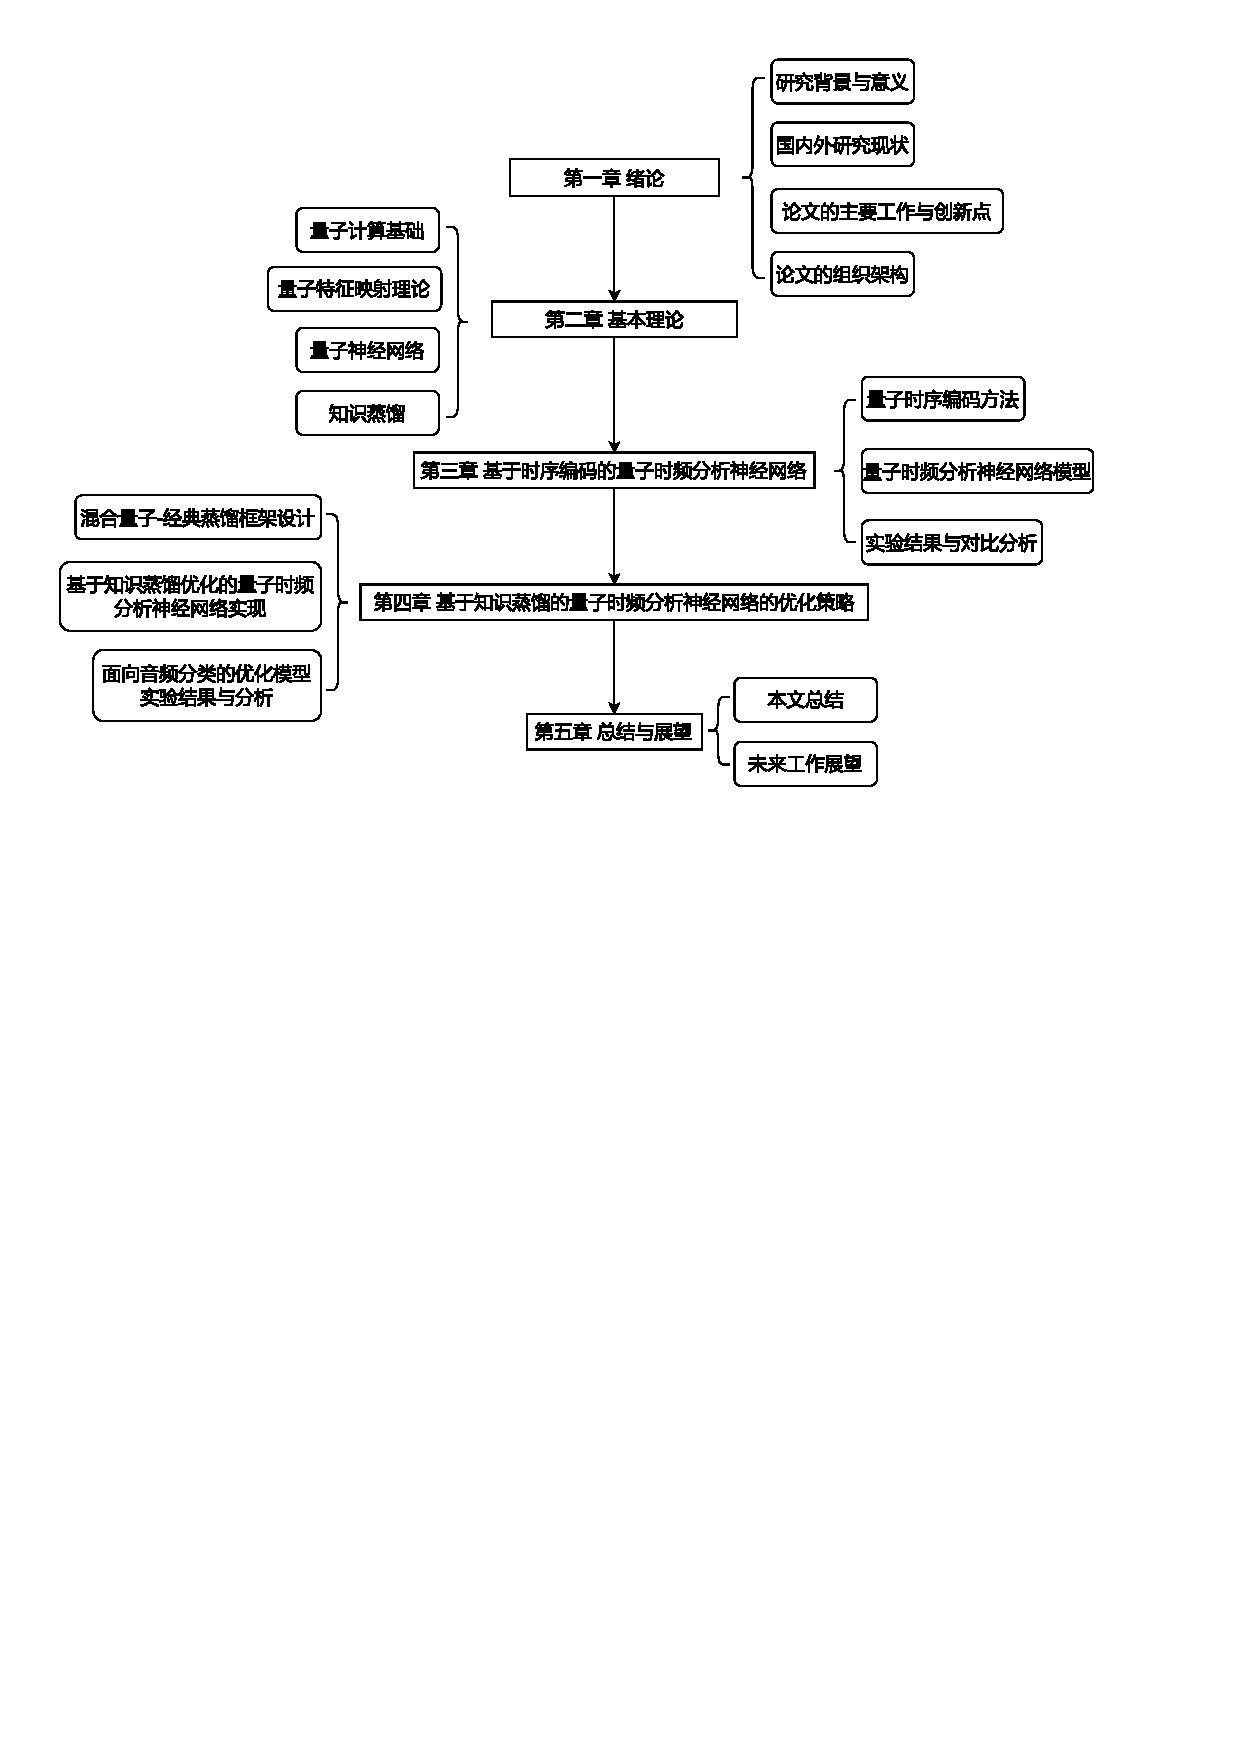
\includegraphics[width=1\textwidth]{./images/The structure of article.pdf}
	\caption{论文组织架构图}
	\label{all}
\end{figure*}

第一章为绪论。首先介绍了基于量子神经网络的音频分类研究背景与深远意义，接着从音频分类任务、量子信息的编码与表示、量子神经网络架构以及模型压缩与知识蒸馏四个方面详细梳理了国内外的研究现状。在剖析现有模型不足的基础上，引出了本文的主要研究内容与创新点，最后对论文的整体组织架构进行了说明。

第二章为相关理论基础。本章系统性地介绍了运用量子机器学习进行音频分类所涉及的核心理论知识，主要涵盖量子计算的基础概念、量子特征映射理论、量子神经网络的基本架构与运行原理，以及知识蒸馏的理论演进。这些内容为后续核心章节中模型的设计与优化奠定了坚实的物理与数学基础。

第三章为基于时序编码的量子时频分析神经网络。本章作为本文的核心方法部分，由数据编码与网络架构两部分紧密结合构成。首先，针对传统量子编码容易丢失音频动态时序特征的局限性，提出了一种基于双量子比特序列纠缠的量子时序编码方案，实现了高频时空特征向高维量子态的高效映射；随后，在此编码机制的基础上，构建了一个端到端的量子时频分析神经网络架构。详细剖析了网络中量子卷积层、量子池化层及测量模块的设计机制，并通过在 GTZAN 基准数据集上开展详尽的对比实验，验证了该模型在极低参数量下依然具备优异的特征提取能力与分类性能。

第四章探讨了基于量子时频分析神经网络的优化。为了克服纯量子网络在复杂特征表征上的局限以及 NISQ 设备下易出现的梯度消失问题，本文引入了知识蒸馏机制，构建了“经典 CNN 教师-量子学生”的异构训练框架。本章详细说明了联合损失函数的数学构造与超参数寻优过程。多维度的指标评估证实，该策略有效改善了网络的收敛稳定性，并一定程度上提升了量子线路的泛化能力与分类下限。

第五章为总结与展望。本章对全文的核心理论与工程成果进行了总结，客观分析了现阶段模型设计中存在的局限性，并结合量子底层硬件与混合算法的发展趋势，对该领域未来的研究方向提出了展望。